\documentclass[conference]{IEEEtran}
\IEEEoverridecommandlockouts%

\usepackage[utf8]{inputenc}
\usepackage[T1]{fontenc}
\usepackage[english,brazilian]{babel}
\usepackage{amsmath}
\usepackage{array}
\usepackage{booktabs}
\usepackage{graphicx}
\usepackage{bookmark}
\usepackage{eso-pic}
\usepackage[section]{placeins}
\usepackage{tikz}
\usepackage{listings}
\usepackage{hyperref}
\usepackage{url}

\hypersetup{colorlinks=true,linkcolor=blue,urlcolor=blue,citecolor=blue}

\lstset{basicstyle=\ttfamily\scriptsize, breaklines=true, columns=fullflexible,
        frame=single, framerule=0.3pt, xleftmargin=0pt, aboveskip=4pt, belowskip=2pt}

% ---------------------------------------------------------------
% Dados do autor
% ---------------------------------------------------------------
\newcommand{\autorNome}{Navinchandry Bittencourt Ruas}
\newcommand{\autorMatricula}{241034353}
\newcommand{\autorEmail}{241034353@aluno.unb.br}

% Marca d'água no fundo de todas as páginas.
\AddToShipoutPictureBG{%
\begin{tikzpicture}[remember picture,overlay]
\node[opacity=0.06,inner sep=0pt] at (current page.center) {
\includegraphics[width=0.48\paperwidth]{figures/unb-logo-square.png}};
\end{tikzpicture}%
}

\title{%

\includegraphics[width=0.95\textwidth]{figures/unb-logo-wide.jpg}\\[-0.8ex]
\vspace{0.4ex}
Montador e Ligador de Duas Passagens para uma Máquina Hipotética: Projeto, Implementação e Validação em C++}

\author{%
\IEEEauthorblockN{\autorNome}
\IEEEauthorblockA{Departamento de Ciência da Computação\\
Universidade de Brasília\\
Matrícula: \autorMatricula\\
\autorEmail}
}

\begin{document}
\maketitle

\begin{abstract}
Este trabalho descreve o projeto e a implementação de um montador de duas passagens e de um ligador para a linguagem simbólica de uma máquina hipotética de 14 instruções, desenvolvidos em C++17 na disciplina CIC0104 --- Software Básico. O montador realiza análise léxica, sintática e semântica, suporta as diretivas \texttt{SPACE}, \texttt{CONST}, \texttt{EQU} e \texttt{IF}, endereçamento \texttt{ROTULO + N} e reporta todos os erros do arquivo, com linha e tipo, antes de gerar o objeto em formato texto. O ligador combina até três módulos, realocando endereços e resolvendo símbolos externos. A validação reuniu 81 verificações automatizadas com resultados esperados calculados à mão, execuções no simulador da disciplina, teste diferencial com 3.000 programas válidos aleatórios e \emph{fuzzing} sob sanitizadores de memória; todas foram bem-sucedidas, e o objeto gerado para o exemplo de referência é idêntico, byte a byte, ao fornecido.
\end{abstract}

\noindent Palavras-chave: montador, ligador, duas passagens, análise léxica, realocação, software básico

\vspace{1\baselineskip}

\begin{otherlanguage}{english}
\begin{abstract}
This paper describes the design and implementation of a two-pass assembler and a linker for the symbolic language of a 14-instruction hypothetical machine, written in C++17 for the CIC0104 Basic Software course. The assembler performs lexical, syntactic and semantic analysis, supports the \texttt{SPACE}, \texttt{CONST}, \texttt{EQU} and \texttt{IF} directives and \texttt{LABEL + N} addressing, and reports every error in the file, with line and type, before emitting a text object. The linker merges up to three modules, relocating addresses and resolving external symbols. Validation combined 81 automated checks with hand-computed expectations, runs on the course simulator, differential testing against 3,000 random valid programs and fuzzing under memory sanitizers; all succeeded, and the object produced for the reference example is byte-identical to the one provided.
\end{abstract}
\noindent Keywords: assembler, linker, two-pass, lexical analysis, relocation, system software
\end{otherlanguage}

% ===============================================================
\section{Introdução}
Montadores e ligadores são a base da cadeia de tradução de programas: o primeiro converte código simbólico em código de máquina e o segundo combina módulos separados em um executável~\cite{beck,levine}. Implementá-los permite fixar conceitos de análise léxica, sintática e semântica, tabelas de símbolos e realocação~\cite{aho}.

O objetivo deste trabalho, proposto no enunciado da disciplina~\cite{enunciado}, é construir em C/C++ (i)~um programa \texttt{montador} que traduz a linguagem simbólica hipotética para um objeto em formato texto, identificando erros léxicos, sintáticos e semânticos, e (ii)~um programa \texttt{ligador} que, chamando internamente o montador, gera um executável \texttt{.LIG} a partir de até três módulos. A implementação, em C++17~\cite{cpp17}, possui cerca de 1.320 linhas, sem dependências externas. O código-fonte está disponível em \url{https://github.com/naviNBRuas/HypoForge}.

% ===============================================================
\section{Fundamentação}
\subsection{A máquina hipotética}
A máquina possui um acumulador e 14 instruções (Tabela~\ref{tab:isa}). Cada instrução ocupa uma palavra de opcode seguida de zero a dois endereços. Programas têm uma seção \texttt{TEXT} (instruções) e uma \texttt{DATA} (\texttt{CONST} e \texttt{SPACE}); no objeto, os dados vêm sempre depois do código.

\begin{table}[!htbp]
\centering
\caption{Instruções da máquina hipotética}\label{tab:isa}
\begin{tabular}{p{2.5cm} p{1.2cm} p{3.3cm}}
\toprule
\textbf{Instrução} & \textbf{Opcode} & \textbf{Tamanho (palavras)}\\
\midrule
ADD, SUB, MULT, DIV & 1--4 & 2\\
JMP, JMPN, JMPP, JMPZ & 5--8 & 2\\
COPY & 9 & 3\\
LOAD, STORE & 10, 11 & 2\\
INPUT, OUTPUT & 12, 13 & 2\\
STOP & 14 & 1\\
\bottomrule
\end{tabular}
\end{table}

\subsection{Montagem em duas passagens}
Referências a rótulos definidos mais adiante impedem a geração imediata de código. O algoritmo de duas passagens resolve isso: a primeira percorre o fonte, avalia o tamanho de cada comando e preenche a tabela de símbolos; a segunda, já com todos os endereços conhecidos, gera as palavras~\cite{beck}.

\subsection{Ligação e realocação}
Módulos são montados independentemente, com endereços relativos ao seu início. O ligador soma a cada módulo uma \emph{base} (soma dos tamanhos dos anteriores) em todas as palavras que representam endereços locais, e preenche as referências a símbolos \texttt{EXTERN} com os endereços definidos por \texttt{PUBLIC} em outros módulos~\cite{levine}.

% ===============================================================
\section{Projeto e Implementação}
\subsection{Visão geral}
O código está organizado em módulos pequenos: tabela de instruções, analisador léxico, montador, formatos de objeto e ligador, compartilhados por dois executáveis. A Figura~\ref{fig:architecture} mostra o fluxo do montador.

\begin{figure}[!htbp]
\centering
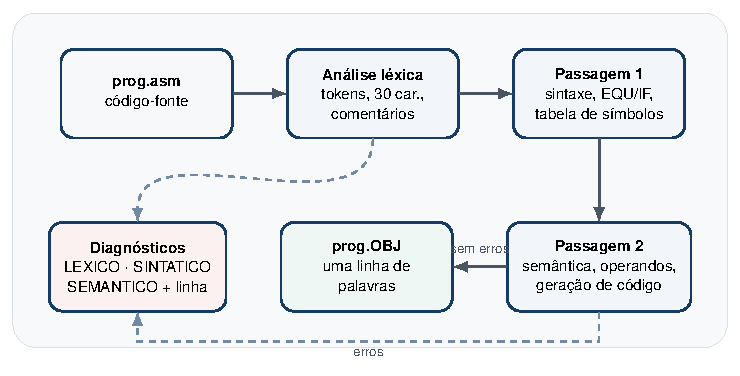
\includegraphics[width=0.98\linewidth]{figures/fig1-arquitetura.pdf}
\caption{Fluxo do montador: análise léxica, duas passagens e geração do objeto; erros são acumulados e exibidos ao final.}\label{fig:architecture}
\end{figure}

\subsection{Análise léxica}
Cada linha é truncada no símbolo \texttt{;} e dividida em identificadores, números e os símbolos \texttt{:}, \texttt{+}, \texttt{-} e vírgula. Identificadores são convertidos para maiúsculas, tornando a linguagem insensível ao caso, e tabulações e espaços extras são ignorados. São erros léxicos: caracteres fora do alfabeto, identificadores com mais de 30 caracteres e tokens iniciados por dígito (como \texttt{1ABC} e \texttt{0x10}, pois \texttt{CONST} aceita apenas decimal).

\subsection{Primeira passagem: sintaxe e símbolos}
Para cada linha reconhece-se \texttt{rotulo:}, o mnemônico e os operandos, verificando a quantidade de operandos. Um rótulo sozinho na linha fica pendente e é associado ao próximo comando. Rótulos são gravados com endereço relativo à seção; \texttt{EQU} é avaliado imediatamente e um \texttt{IF} falso descarta a linha seguinte. Linhas com erro léxico não recebem análise sintática adicional, evitando erros em cascata.

\subsection{Segunda passagem: semântica e código}
Com o tamanho do texto conhecido, rótulos de dados recebem \texttt{endereço + tamanho do texto}, o que permite que a seção \texttt{DATA} venha antes ou depois de \texttt{TEXT}. Operandos \texttt{ROTULO + N} são resolvidos e as verificações semânticas são aplicadas (Tabela~\ref{tab:errors}). O arquivo inteiro é sempre analisado; os erros são ordenados por linha e, havendo algum, nenhum \texttt{.OBJ} é gravado.

\begin{table}[!htbp]
\centering
\caption{Erros detectados por classe}\label{tab:errors}
\begin{tabular}{p{2.1cm} p{4.9cm}}
\toprule
\textbf{Classe} & \textbf{Exemplos}\\
\midrule
LEXICO & caractere inválido; identificador $>$ 30; token iniciado por dígito\\
SINTATICO & nº de operandos errado; instrução/diretiva inválida; vírgula em \texttt{COPY}; dois rótulos\\
SEMANTICO & rótulo ausente ou repetido; \texttt{TEXT} ausente; escrita em \texttt{CONST}; salto para dado; acesso além da área reservada por \texttt{SPACE}/\texttt{CONST}; divisão por constante 0; \texttt{BEGIN} sem \texttt{END}\\
\bottomrule
\end{tabular}
\end{table}

\subsection{Formato dos objetos e ligador}
O objeto do montador é uma linha de palavras separadas por espaço, programa primeiro e depois dados, idêntica ao formato do exemplo de referência. Quando chamado pelo ligador (opção \texttt{--modular}), o montador acrescenta tabelas de definições (\texttt{D}), usos externos (\texttt{U}) e um bit de realocação por palavra (\texttt{R}). O ligador (i)~calcula as bases, (ii)~monta a tabela global de símbolos, (iii)~soma a base às palavras marcadas e (iv)~soma o endereço global do símbolo a cada uso externo. Definições duplicadas e externos indefinidos abortam a ligação. A Figura~\ref{fig:linking} ilustra o resultado para o exemplo de dois módulos.

\begin{figure}[!htbp]
\centering
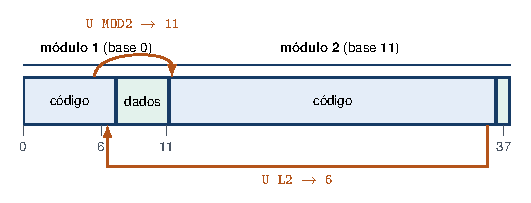
\includegraphics[width=0.98\linewidth]{figures/fig2-ligacao.pdf}
\caption{Disposição do executável ligado (37 palavras) e as duas referências externas resolvidas.}\label{fig:linking}
\end{figure}

% ===============================================================
\section{Testes e Resultados}
\subsection{Metodologia}
A suíte (\texttt{make test}) é composta por 81 verificações (Tabela~\ref{tab:tests}). Para programas válidos, o objeto é comparado byte a byte com expectativas calculadas à mão, e o exemplo fornecido é comparado com o objeto de referência. Para programas inválidos, compara-se a lista de pares linha/tipo de erro. Programas montados e ligados são executados no simulador da disciplina, e a linha de comando é testada com nomes com pontos, espaços e extensão maiúscula, argumentos errados e remoção de saídas antigas.

Os casos incluem entradas \emph{armadilha}: rótulo sozinho seguido de comentários e linhas vazias, identificadores com 30 e 31 caracteres, \texttt{X+1} sem espaços, \texttt{COPY A,B}, constantes hexadecimais, fracionárias e fora do intervalo, acentos, palavras reservadas como rótulo, \texttt{IF} aninhado, BOM UTF-8 e finais de linha CRLF ou CR. Em \texttt{make stress}, um teste diferencial compara 3.000 programas válidos aleatórios com objetos calculados de forma independente, e um \emph{fuzzer} submete 6.000 programas e 600 ligações aleatórias; com AddressSanitizer e UBSan, não houve travamentos nem erros de memória.

\begin{table}[!htbp]
\centering
\caption{Resumo da suíte de testes}\label{tab:tests}
\begin{tabular}{p{2.6cm} p{0.9cm} p{3.2cm}}
\toprule
\textbf{Categoria} & \textbf{Casos} & \textbf{Resultado}\\
\midrule
Programas válidos & 25 & objeto idêntico\\
Programas inválidos & 28 & linhas e tipos corretos\\
Ligação & 13 & \texttt{.LIG}, saída e erros\\
Simulador & 6 & saída esperada\\
Linha de comando & 9 & nomes, códigos de saída\\
\midrule
\textbf{Total} & \textbf{81} & \textbf{81 aprovados}\\
\bottomrule
\end{tabular}
\end{table}

\subsection{Montagem de um programa válido}
O programa \texttt{bin.asm} lê um inteiro e imprime seus dígitos binários (do menos significativo ao mais). O objeto gerado coincide com o de referência:
\begin{lstlisting}
$ ./montador examples/bin.asm
Montagem concluida: examples/bin.OBJ (32 palavras)
$ cat examples/bin.OBJ
12 29 10 29 4 28 11 30 3 28 11 31 10 29 2 31 11 31
13 31 9 30 29 10 29 7 4 14 2 0 0 0
\end{lstlisting}

\subsection{Detecção de erros}
Para o exemplo do enunciado, em que o rótulo \texttt{N3} não é declarado, todas as ocorrências são reportadas em uma única execução:
\begin{lstlisting}
[ERRO SEMANTICO] linha 11: rotulo 'N3' nao declarado
    11 | COPY N2 N3
[ERRO SEMANTICO] linha 12: rotulo 'N3' nao declarado
    12 | COPY N3 N3
[ERRO SEMANTICO] linha 13: rotulo 'N3' nao declarado
    13 | OUTPUT N3
\end{lstlisting}

\subsection{Ligação de módulos}
O módulo~1 lê o número e salta para \texttt{MOD2}; o módulo~2 executa o laço e retorna a \texttt{L2}. O executável ligado produz as mesmas saídas que o programa de módulo único para todas as entradas testadas (por exemplo, 13 gera 1, 0, 1, 1):
\begin{lstlisting}
$ ./ligador examples/modulo1.asm examples/modulo2.asm
  modulo examples/modulo1.asm: base 0, 11 palavras
  modulo examples/modulo2.asm: base 11, 26 palavras
Ligacao concluida: examples/modulo1.LIG (37 palavras)
\end{lstlisting}
Também foi testado um caso com três módulos (soma de uma constante a um valor lido) e casos de erro de ligação.

% ===============================================================
\section{Discussão}
\subsection{Decisões de interpretação}
O enunciado deixa pontos em aberto, resolvidos como segue. As palavras \texttt{SECAO} e \texttt{SECTION} são aceitas, pois o texto e os exemplos divergem. \texttt{COPY} com vírgula é erro sintático, já que os arquivos de teste não serão corrigidos. \texttt{CONST} hexadecimal é erro léxico (apenas decimal). O objeto termina com um espaço após cada palavra, sem quebra de linha final, reproduzindo o exemplo fornecido. \texttt{END} não interrompe a leitura, pois o exemplo de módulo posiciona \texttt{SECTION DATA} depois dele. Além das seis classes de erro listadas no enunciado, foram implementadas verificações clássicas (escrita em constante, divisão por constante zero, tipo de rótulo incompatível, acesso além da área reservada). BOM UTF-8 e finais de linha apenas com CR são aceitos, e uma execução com falha remove \texttt{.OBJ} ou \texttt{.LIG} antigos deixados por uma execução anterior.

\subsection{Inconsistências nos exemplos}
O objeto modular de exemplo do curso informa \texttt{L2} no endereço 7, mas a instrução \texttt{STOP} rotulada está no endereço 6; nomeia \texttt{TEMP\_DATA} um símbolo declarado como \texttt{TMP\_DATA}; e traz 9 bits de realocação para 11 palavras. O formato modular aqui adotado mantém o mesmo esquema \texttt{D/U/R}, mas com um bit por palavra e endereços conferidos.

\subsection{Limitações}
O ligador aceita no máximo três módulos, conforme o enunciado, e assume que a execução começa no primeiro módulo. Os limites de \texttt{ROTULO + N} são verificados apenas para dados locais; um deslocamento aplicado a um símbolo \texttt{EXTERN} não pode ser verificado pelo montador.

% ===============================================================
\section{Conclusões}
Foram implementados um montador de duas passagens e um ligador que cumprem a especificação: saída em formato texto com o nome do arquivo trocado para \texttt{.OBJ}, análise completa do arquivo com erros por linha e tipo, suporte a \texttt{EQU}/\texttt{IF} e ligação de até três módulos com realocação. A validação automatizada e o uso do simulador da disciplina indicam comportamento correto nos cenários cobertos, inclusive a identidade byte a byte com o objeto de referência.

Como trabalho futuro, sugere-se: (i)~verificação, na ligação, dos limites de deslocamentos externos; (ii)~um modo de listagem com endereços e código lado a lado; e (iii)~um ponto de entrada configurável no ligador.

% ---------------------------------------------------------------
% REFERÊNCIAS
% ---------------------------------------------------------------
\begin{thebibliography}{10}
\bibitem{aho} A. V. Aho, M. S. Lam, R. Sethi and J. D. Ullman, \emph{Compilers: Principles, Techniques, and Tools}, 2nd ed. Pearson Addison-Wesley, 2006.
\bibitem{beck} L. L. Beck, \emph{System Software: An Introduction to Systems Programming}, 3rd ed. Addison-Wesley, 1997.
\bibitem{levine} J. R. Levine, \emph{Linkers and Loaders}. Morgan Kaufmann, 1999.
\bibitem{enunciado} Universidade de Brasília, Departamento de Ciência da Computação, ``Trabalho Prático 1 --- CIC0104 Software Básico, turma T02,'' enunciado da disciplina.
\bibitem{cpp17} ISO/IEC 14882:2017, \emph{Programming Languages --- C++}, 2017.
\end{thebibliography}

\end{document}
